\documentclass[a4paper,oneside,11pt]{report}
\usepackage{amsmath,algpseudocode,fancyhdr,float,geometry,graphicx,titlesec}
\usepackage{hyperref}
\usepackage[all]{hypcap}

%----------------------- Macros and Definitions --------------------------
\setlength{\headheight}{20pt}
\addtolength{\topmargin}{-10pt}
\addtolength{\textheight}{45pt}
\addtolength{\footskip}{20pt}

\everymath{\displaystyle}

% style for title page
\fancypagestyle{empty}{%
\fancyhf{}
\fancyhead[L]{\large Eindhoven University of Technology}
\fancyhead[R]{\large 2IO70 DBL Embedded Systems}
\fancyfoot[C]{\large Department of Mathematics and Computer Science}
\renewcommand{\headrulewidth}{0pt}
\renewcommand{\footrulewidth}{0pt}
}

% style for \chapter pages
\fancypagestyle{plain}{%
\fancyhf{}
\fancyhead[L]{\large Eindhoven University of Technology}
\fancyhead[R]{\large 2IO70 DBL Embedded Systems}
\fancyfoot[L]{\large Department of Mathematics and Computer Science}
\fancyfoot[R]{\large\thepage}
\renewcommand{\headrulewidth}{1pt}
\renewcommand{\footrulewidth}{0pt}
}

% style for other pages
\pagestyle{fancy}
\fancyhf{}
\fancyhead[L]{\large Eindhoven University of Technology}
\fancyhead[R]{\large 2IO70 DBL Embedded Systems}
\fancyfoot[L]{\large Department of Mathematics and Computer Science}
\fancyfoot[R]{\large\thepage}
\renewcommand{\headrulewidth}{1pt}
\renewcommand{\footrulewidth}{0pt}

% change the chapter formatting
\titleformat
{\chapter} % command
[hang] % shape
{
    \titleline[c]{\titlerule[.8pt]}
    \vspace{0pt}
    \bfseries\LARGE
    \centering
} % format
{\thechapter\quad} % label
{0.0pt} % sep
{} % before-code
[
\vspace{1ex}
\titleline{\titlerule[.8pt]}
] % after-code

% display "Table of Contents" instead of "Contents"
\renewcommand{\contentsname}{Table of Contents}

% get rid of annoying auto-indents
\newlength\tindent                          % make new length variable
\setlength{\tindent}{\parindent}            % set variable to current indent length
\setlength{\parindent}{0pt}                 % set default indent length to 0
\renewcommand{\indent}{\hspace*{\tindent}}  % make manual indent command if indents are wanted.

% set spacing between paragraphs
\setlength{\parskip}{6pt}

% make enumerate compact
\let\oldenumerate\enumerate
\renewcommand{\enumerate}{
\oldenumerate
\setlength{\itemsep}{0pt}
}

% make itemize compact
\let\olditemize\itemize
\renewcommand{\itemize}{
\olditemize
\setlength{\itemsep}{0pt}
}

\newcommand{\comment}[1]{}

%-------------------------------- Title ----------------------------------
\title{\bfseries\huge Sort It Out \\ \LARGE \hfill \\ Final Report}
\author{\begin{tabular}{r c l}
Aleksandr Popov & 0924595 & \texttt{a.popov@student.tue.nl}\\
Dan Cristian Chirascu & 0923784 & \texttt{d.c.chirascu@student.tue.nl}\\
Devin van Broekhoven & 0839004 & \texttt{d.v.broekhoven@student.tue.nl}\\
Jiddo van Vliet & 0821894 & \texttt{j.g.v.vliet@student.tue.nl}\\
Yuntao Li & 0910663 & \texttt{y.li.2@student.tue.nl}
\end{tabular}}

\date{\today}


%--------------------------------- Text ----------------------------------
\begin{document}
% fix hyperref numbering issues
\pagenumbering{Alph}
\maketitle
\pagenumbering{arabic}

%%------------------------------------------------------------------------------------------------------%%
%%--------------------------------------------Summary/Abstract------------------------------------------%%
%%------------------------------------------------------------------------------------------------------%%
%%------------------------------------------------------------------------------------------------------%%
\chapter*{Summary}
Project "DBL 2IO70" concerns specification, design and construction of a sorting machine using a microcontroller, namely, Practicum Processor 2 (PP2). This document is the Final Report for the project, describing in detail each phase of the project conducted by group 17 and the outcomes of each phase, including motivation of design choices in both hardware and software and various correctness proofs and testing details.

\tableofcontents

\chapter{Introduction}
This document encompasses all the work that has been done by Group 17 on the project 2IO70 DBL Embedded Systems. The project involves building, programming and testing the sorting machine, documenting every phase and validating and explaining the design choices formally.

During the project our group has worked on different aspects on designing, building and programming the sorting machine. These aspects are:
\begin{itemize}
\item Machine design, making an overall design of the machine and explaining under which circumstances the machine can be operated. In this part also the safety properties and user constraints are explained.
\item Software specification as the first step of integrating the PP2 processor into the machine. We explained which inputs and outputs we will use and how they are related to each other.
\item Software design, requiring us to write Java-syntax pseudocode. This code was used to give an general layout of the PP2 Assembly program for the PP2 processor.
\item Software implementation and integration as the phase where we had to write PP2 Assembly code for the machine. At the end of this phase our sorting machine had to be fully functional.
\item System validation and testing, requiring us to use different means to test our software and hardware. We had to explain our code and show that it could handle all the test cases that corresponded to use cases.
\end{itemize}

These parts were divided into further sections that helped to maintain a structural sequential approach in building the machine. Detailed information about each section of the project can be found in this Final report.

%%------------------------------------------------------------------------------------------------------%%
%%-------------------------------------Copy of Assignment Description-----------------------------------%%
%%------------------------------------------------------------------------------------------------------%%
%%------------------------------------------------------------------------------------------------------%%
\chapter{The Project Assignment}
This part of the report contains the copy of project assignment, describing the requirements placed on the machine, in order for the reader to have a clear concept of what had to be done and what is done.

\section{Introduction}
The subject of the Design Based Learning project “DBL 2IO70” is specification, design and construction of a machine that is controlled by a so called microcontroller. A microcontroller is a very small computer that is equipped with inputs and outputs that can be used to control a machine. Since the microcontroller does not operate in a stand-alone fashion, like a personal computer does, but is a part of a larger whole --- the machine thus controlled --- such a controller including its software is called an embedded system. In one very important aspect, however, a microcontroller is a real computer: it operates under the control of a program. The design and construction of an embedded system, therefore, unavoidably involves programming.

In this project methods and techniques are used to which the participants have been introduced during the preceding quartile. In particular, the project elaborates on the knowledge and experience with (the programming of) microcontrollers obtained in the Computer Systems course.

In this project the participants also have to solve problems of a mechanical or electrical nature, which cannot be considered as true software engineering problems, but which a software engineer may encounter in an industrial environment. In this respect this project clearly has a multi-disciplinary flavour.

\section{The Sorting Machine}
The goal of this project is to build a simple sorting machine that is able to separate small objects, plastic discs that may be either black or white, into two sets: the black discs and the white discs. For this purpose the machine is equipped with, among other things, one or two conveyor belts to transport the discs inside the machine. Initially the discs to be sorted are contained in a storage tube; the machine will have a mechanism to deposit one disc at a time onto a conveyer belt.

The intended sorting process now proceeds as follows. From the storage tube a disc is deposited onto the first conveyor belt. This belt transports the disc to a so called black/white detector. Arrival of the disc at this detector is to be signaled; this can be done by means of a so called light trap, which consists of a lamp and a photo cell: arrival of the disc is detected by interruption of the light beam from the lamp to the photo cell.

The black/white detector itself also consists of a lamp and a photo cell, but these are positioned in such a way that the photo cell measures the light that is reflected by the disc: as white discs reflect considerably more light than black ones, white and black discs can thus be distinguished.

Subsequently, the disc is transported further to one of two trays in which the black and white discs are collected: one tray for the black discs and one tray for the white ones. These trays may, for instance, be positioned at the two ends of the conveyor belt, or a second conveyor belt may be used for this purpose. So, depending on its design, the machine may have two conveyor belts, or just a single one. In either case, in which of the two trays a disc is deposited depends on the direction of movement of the conveyor belt, which is to be determined by the microcontroller; this direction, of course, will depend on the measurement provided by the black/white detector.

See Figure \ref{fig:exampledesign} for a possible general layout of the machine, in the case of a machine with two conveyor belts. (In this drawing the mechanism to deposit a disc from the storage tube onto the conveyor belt has not been drawn.)

Of course, other configurations are possible (and permitted) too; the black/white detector, for example, could also be placed above the second conveyor belt --- does that have advantages? And as already suggested above, a machine containing a single conveyor belt only is conceivable, too. The only real requirement is that the machine must contain at least one conveyor belt.
\begin{figure}[H]
\centering
\includegraphics[width=0.9\textwidth]{images/exampledesign.jpg}
\caption{Possible Layout of the Machine}
\label{fig:exampledesign}
\end{figure}

\section{Control Buttons and Details of the Process}
The machine is to be operated by means of two push buttons, called “START/STOP” and “ABORT”, in the following way. This process description is based on a machine configuration with two conveyor belts and with the black/white detector above the first belt, as in Figure \ref{fig:exampledesign}. For other configurations this process description must be rewritten accordingly. The two push buttons “START/STOP” and “ABORT” may be simply realised by dedicating two of the (eight) push buttons on the PP2 board to
this purpose.

\begin{enumerate}
\item After starting the program in the microcontroller the machine is in its resting state. In this state black and white discs can be placed manually into the storage tube. In the resting state all motors in the machine are stopped and all lamps are off.
\item By pressing button “START/STOP” the machine is started and proceeds to its regular operating state. First, if necessary, the machine brings all internal mechanisms into their well-defined initial state.
\item After this the actual sorting process starts. The machine deposits one disc onto the first conveyor belt, after which this belt transports the disc to the black/white detector. Then the belt stops and the color of the disc is measured by means of the detector.
\item If the storage tube was empty then obviously no disc was deposited onto the conveyor belt and the presence detector at the black/white detector will never signal arrival of a disc. “Never”, however, takes a very long time and, therefore, it is impossible to decide that something “never” happens. Based on knowledge of the speed of the conveyor belt it is possible to calculate when arrival of the disc at the black/white detector is to be expected. If 4 seconds after this expected arrival time the presence detector has not signaled the arrival of a disc, then we assume that such a disc will indeed never arrive because the storage tube was empty. If this happens the machine stops and returns to its resting state. In this way the sorting process will terminate automatically after all discs from the storage tube have been processed.
\item If the presence detector at the black/white detector does signal arrival of a disc, the second conveyor belt starts moving into the direction of the correct collecting tray depending on the observed color of the disc. As the disc is still on the first conveyor belt, this belt is started again, too, in order to transport the disc to the second belt.
\item In order to detect that the disc really reaches a tray, additional light traps must be placed at both ends of the second conveyor belt. (In Figure \ref{fig:exampledesign} these additional detectors have not been drawn.)
\item If the disc has been deposited into the right tray the machine repeats the cycle that starts with placing a disc onto the first conveyor belt; that is, the machine returns to step 3 and continues operating in this way until the process terminates because the supply of discs is exhausted, as described in step 4.
\item If during the sorting process the push button “START/STOP” is pressed the machine completes the current cycle, that is, the machine continues its normal operation until the current disc has been deposited into the correct tray. Then the machine stops and returns to its resting state. If such a “stop” command has been given, repeatedly pressing the button “START/STOP” again while the machine is still busy completing its current cycle will have no effect whatsoever. If after a “stop” command the machine has completed its cycle and has reached its resting state then the machine is ready again to be started: in this state pressing push button “START/STOP” will start the machine again, just as in step 2.
\item Push button “ABORT” is used as an emergency button. Pressing this button while the machine is in its resting state has no effect. Pressing this button while the machine is operating makes the the machine halt immediately: Both the conveyor belts and the mechanism to deposit discs onto the belt and, possibly, all other mechanisms present in the machine are switched of immediately. The purpose of button “ABORT” is to be able to halt the machine if the person operating it observes that something goes wrong or is about to go wrong. If the machine has been halted this way manual interaction by the operator is needed, for instance, to remove any disc still on a conveyor belt or to remove discs that might have fallen off a conveyor belt --- a most undesirable situation, of course. If, subsequently, the push button “START/STOP” is pressed once, the machine returns to its resting state.
\item To be able to guarantee that the mechanism depositing discs onto the conveyor belt stops in a well-defined state this mechanism must be equipped with (at least) one switch to signal that this mechanism has reached the correct state.
\item It is recommended to make the different operating states of the machine visible on the LEDs and/or the display of the PP2 board. In particular, it is a definite plus if the software controlling the process is designed so as to display the number of black discs and the number of white discs deposited in their corresponding trays.
\end{enumerate}

A general design rule is that motors and lamps are switched off whenever possible, that is, whenever there is no need for them to be switched on.

\section{The Black/White Detector}
The construction of the black/white detector requires some care and some experimenting. After all, the light reflected from a white disc is weaker than direct light; therefore, detecting reflected light is more difficult. For this detector one uses one (or even two!) lens lamps positioned in such a way that it projects a nice patch of light onto the disc to be examined. Then a photo cell is placed in such a way that it “observes” this patch of light. This works best if lamp and photo cell are placed as close as possible to the disc. See Figure \ref{fig:examplebwdet} for a possible configuration.
\begin{figure}[H]
\centering
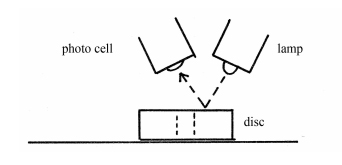
\includegraphics[width=0.4\textwidth]{images/examplebwdet.jpg}
\caption{Possible Configuration of Black/White Detector}
\label{fig:examplebwdet}
\end{figure}

The problem is to make sure that a white disc reflects enough light to be detectable; to make sure that a black disc reflects so little light that it is not seen as a white disc is no problem at all. The correct placement of lamp(s) and photo cell is best determined experimentally. One connects a lens lamp --- with a series resistor, as prescribed in the Technical Guide --- to the 12 V connector on the PP2 board. Also, one connects a photo cell --- also as prescribed in the Technical Guide --- to one of the digital inputs of the PP2 board. The PP2 board then is powered, but does not need a program: the green LED corresponding to the digital input of the photo cell will indicate the state of that input.

Now place a white disc under the detector under construction and position lamp and photo cell in such a way that the green LED at the input lights up. That means that the white disc is recognized. Make sure that this works correctly, even with minor variations in the positions of the disc, the lamp and the photo cell. If you are satisfied with the result then secure the positions of the lamp and the photo cell. Finally, place a black disc under the detector and verify that it is not seen as white.

To prevent surrounding light disturbing the measurement a black shielding hood can be placed over the photo cell.

It is also possible to use one of the two A/D inputs --- again: see the Technical Guide how to do this --- of the PP2 board. This makes construction of the black/white detector easier, and it is even possible to use a single lamp and photo cell combination both as a presence detector and as a black/white detector. The use of A/D converters in situations where they are not really needed, however, is considered a wasteful use of resources. Therefore, the use of an A/D input is permitted but it is a definite plus if the A/D inputs are not used and the black/white detector uses digital inputs only. (This is possible!)

%%------------------------------------------------------------------------------------------------------%%
%%--------------------------------------------Method of Working-----------------------------------------%%
%%------------------------------------------------------------------------------------------------------%%
%%------------------------------------------------------------------------------------------------------%%
\chapter{Method of Working}
The project for designing, building and documenting the sorting machine is done in phases. Each phase focuses on a different aspect of building or designing the machine. The phases of the project are:
\begin{enumerate}
\item Machine design
\item Software specification
\item Software design
\item Software implementation
\item System validation and testing
\end{enumerate}

In the machine design phase the actual machine has to be built using the Fisher Technik parts. Also the use cases, user constraints and safety properties have to be described. This was done entirely during the group meetings. Therefore, the workload was equally distributed in an informal way. Most mechanical operations, however, can be attributed to Devin van Broekhoven.

The software specification part was done with an informal distribution of the workload as well, as we completed the entire document and the UPPAAL model during our group meetings. However, most work on the document has been done by Jiddo van Vliet, and most work on the UPPAAL model --- by Yuntao Li and Aleksandr Popov.

Software design was done in two groups, where one group was responsible for the Java code (Aleksandr Popov, Dan Cristian Chirascu) and the other was responsible for writing all the necessary documentation about the Java code. Large parts were later added to the document and reviewed by Aleksandr Popov.

The software implementation phase included writing the Assembly language program to control our machine. The Assembly language program was divided into multiple sections which represented the states of the machine. Each member of the group had to write a certain part of the program. After all parts were done, they were combined and checked for errors. Large parts have been rewritten in order to correct errors and integrate them into the program. Most credit here can be attributed to Aleksandr Popov.

System validation and testing phase implies demonstrating that the final product meets its initial requirements, that is, that the executable object code correctly implements the System Level Requirements. Also, it is important to show that the implementation does not do more than expected. In this phase we had to do both code review and formal proofs. For code review, we elected a presenter to show the code and the other members did the check and gave feedback. For formal proofs we relied on our UPPAAL model to check if the safety properties were correctly implemented. Verification of the UPPAAL model has mostly been done by Yuntao Li.

Finally, all the documents were reviewed, formatted and incorporated into this document. This work can be attributed to Devin van Broekhoven and Aleksandr Popov.

%%------------------------------------------------------------------------------------------------------%%
%%---------------------------------------------Machine Design-------------------------------------------%%
%%------------------------------------------------------------------------------------------------------%%
%%------------------------------------------------------------------------------------------------------%%
\chapter{Machine Design}
This part of the report describes the process of designing the sorting machine for the project 2IO70 DBL Embedded Systems. It includes motivation of certain design choices and the description of the machine layout, but also the sub-documents "System Level Requirements" and "Machine Interface".

\section{Machine Layout. Motivating the Design Choices}
For the system to be easy to use and for us to be able to easily fix emerging problems we decided to design the machine on multiple levels. The first component of the machine is the loading tube and the dispenser --- the mechanism to push one disc at a time onto the conveyor belt. It also includes the black/white detector, presence detector and a button located next to dispenser that is used to reliably determine its current position. This component is located on top of the machine so that the user can easily load the discs into the loading tube. The second component of the machine includes the conveyor belt, two trays for the discs and two side presence detectors that are used to determine whether a certain disc has indeed reached the tray and no exceptional situations have occurred.

To keep the machine as fast as possible we decided to identify the color of the disc before it is loaded onto the conveyor belt. This way we can ensure the disc keeps moving when it has left the loading tube and thus no time is wasted during the sorting process. Since identifying the color of a disc using the sensors included in the kit is nearly instant we were able to integrate the black/white detector into the component which pushes the disc on the conveyor belt.

After a disc has passed the black/white detector it will be pushed on the conveyor belt. As the conveyor belt itself is located on a lower level and is parallel to the dispenser mechanism, the disc will simply drop down onto the belt. This means that the component which pushes a disc from the loading tube to the conveyor belt can run on a higher speed without the risk of the disc falling sideways.

The conveyor belt is powered by a single engine which is able to turn both ways using the PP2 processor to change the polarity. Based on the input from the black/white detector the conveyor belt will either turn left or right to deliver the disc to its appropriate storage box. We decided to employ presence detectors on both ends of the conveyor belt to detect if a disc has actually been delivered to its storage box. If the detector does not detect a disc on time, the machine aborts the execution of further processes.

\newpage

\section{System Level Requirements}
This part of the document describes the possible use cases, user constraints and safety properties.

\subsection{Use Cases}
General description of sorting process:
\begin{itemize}
  \item \textbf{Pre-condition}\\
  The PP2 processor is connected to all the engines, lights and sensors used in the machine according to the input/output map described in further documents. It is also connected to a computer, and the required program code is properly loaded. There are no discs in the loading tube or on the conveyor belt. No discs or other parts are blocking the moving parts of the machine.
  \item \textbf{Trigger}\\
  The user powers up and initialises the sorting machine by pressing the Start/Stop button and loads all the discs into the loading tube. After that the Start/Stop button is pressed again to start the sorting process.
  \item \textbf{Guarantee}\\
  The machine will start correctly sorting the black and white discs which were inserted into the loading tube.
\end{itemize}

\textbf{Sorting under Normal Conditions}
\begin{enumerate}
\item Pressing the Start/Stop button on the machine puts all mechanical parts in their appropriate resting states. The conveyor belt is stopped and all lights and detectors are turned on. The part which pushes the single discs from the loading tube onto the conveyor belt turns to its most retracted state.
\item The discs are inserted via the loading tube on top of the machine. When all discs are inserted, the user is allowed to press the Start/Stop button again.
\item Pressing the Start/Stop button starts the sorting process.
\item First the machine detects if there are discs left to sort by means of the presence detector.
\item If a disc has been detected it is pushed to the black/white detector which decides which way the conveyor belt should turn.
\item After the color of the disc has been determined the disc is pushed onto the conveyor belt.
\item The conveyor belt transports the disc to one of the two storage boxes depending on the color of the disc.
\item At the end of each side of the conveyor belt a light detector determines if the disc has indeed been delivered to the appropriate storage box in given time limit.
\end{enumerate}

\textbf{Sorting under Deviated Circumstances}
\begin{itemize}
\item A disc fell off (is stuck on) the conveyor belt
    \begin{description}
        \item[8-a] Disc has not been detected by the corresponding side detector in the appropriate time. Abort all operations and go to the halting state. User intervention is needed to recover the lost disc(s).
        \item[8-b] Continue at the first state.
    \end{description}

\item The disc dispenser does not work properly
    \begin{description}
        \item[5-a] User detects malfunctioning of the machine which pushes the discs to the conveyor belt. The user has to press the Abort button.
        \item[5-b] The machine halts immediately, the user has to remove all discs from the system and fix the malfunctioning part.
        \item[5-c] Continue at the first state.
    \end{description}
    \textit{Alternative}
    \begin{description}
        \item[8-a] Disc has not been detected by the corresponding side detector in the appropriate time. Abort all operations and go to halting state. User intervention is needed to remove all discs from the system and fix the malfunctioning part of the machine.
        \item[8-b] Continue at the first state.
    \end{description}

\item The conveyor belt engine is malfunctioning
    \begin{description}
        \item[7-a] User detects malfunctioning of the engine which powers the conveyor belt. The user has to press the Abort button.
        \item[7-b] The machine halts immediately, the user has to remove all discs from the system and fix the malfunctioning engine.
        \item[7-c] Continue at the first state.
    \end{description}
    \textit{Alternative}
    \begin{description}
        \item[8-a] Disc has not been detected by the corresponding side detector at one of the trays in time. Abort all operations and go to halting state. User intervention is needed to remove all discs from the system and fix the malfunctioning engine.
        \item[8-b] Continue at the first state.
    \end{description}
\end{itemize}

\subsection{User Constraints}
\begin{enumerate}
\item The user is only allowed to load the discs into the loading tube when the machine is in its resting state, after initialisation (the Start/Stop button has been pressed once, all lights are on, engines are off). The discs should be loaded with the flat part pointing to the top to avoid possible jamming that might happen due to configuration of loading tube and discs otherwise.
\item When the machine is running the user is not allowed to touch or move the discs.
\item When the user has pressed the Start/Stop button while the machine is running it will finish its current cycle and then go to its resting state. Pressing the Start/Stop button multiple times while it is running will have no effect.
\item When the user has pressed the Abort button the machine will stop immediately (within 15 ms). All discs which have left the loading tube have to be removed and reinserted into the loading tube (see 1. for loading constraints).
\item While the machine is running the user is not allowed to touch any of the components of the machine and should make sure none of the lights and sensors are blocked.
\end{enumerate}

\subsection{Safety Properties}
\textbf{Inputs (in order of use in a cycle)}
\begin{itemize}
\item Dispenser button
\item Presence detector
\item Black/white detector
\item Side presence detector white
\item Side presence detector black
\end{itemize}

\textbf{Outputs (in order of use in a cycle)}
\begin{itemize}
\item Power engine dispenser
\item Power light presence detector
\item Power light black/white detector
\item Power engine conveyor belt
\item Power light presence detector white
\item Power light presence detector black
\end{itemize}

\textbf{Input and output relations}
\begin{itemize}
\item None of the detectors can detect a disc at the same time.
\item The engine for the belt can never run in both directions at the same time.
\item When the Start/Stop button is pressed during a cycle the machine will only stop if the cycle has finished.
\item When the Abort button is pressed all operations have to stop and the machine will go to its halting state. Even when the machine is mid cycle, so for example a disc is on the conveyor belt, the machine has to stop. When the user wants to start the machine again user intervention is necessary to remove any discs from the machine. The halting should take no more than 15 ms.
\item When the presence detector has given a low signal either the black tray or white tray side presence detector should give a low signal before the dispenser finishes its rotation.
\end{itemize}

\newpage

\section{Machine Interface}
The sorting machine is connected to the PP2 board, which plays a role of a microcontroller in this assignment, through a so-called machine interface. In this document every connection between the actual machine and the microcontroller is described briefly.

\begin{itemize}
\item \textbf{Motors}\\
    Two electrical motors are used in the machine. Let them be denoted as motor A and motor B for convenience. Motor A is responsible for the work of the disc supply mechanism, whereas motor B brings the conveyor belt in motion in one of the directions.

    Motor A is connected by a wire of type A to digital output 0 of the PP2, and motor B is connected by a similar wire to the H-bridge between outputs 6 and 7. That enables us to turn motor B in both directions so that we can bring the conveyor in motion in the correct direction and the disc can be deposited in the corresponding tray. When output 6 is high, the conveyor belt turns right; when output 7 is high, it turns left. These two outputs are not allowed to be high simultaneously. However, it does not matter in which direction motor A turns, so it is only connected to 1 output. Polarity in case of motor A does not matter as well.

\item \textbf{Lamps}\\
    Every lamp is connected to a digital output on the PP2. They need to be turned on for the detectors to work (high output on corresponding digital output of the PP2). Polarity does not matter for the lamps. Lamp for the black/white detector is connected to PP2 board (output 2) using a wire of type B to limit the voltage. All the other lamps are connected in series to avoid taking too much current from the PP2 to output 3 by means of a wire of type A.

\item \textbf{Phototransistors}\\
    Phototransistors are used as detectors of (reflected) light from the lamps. In order for them to produce results, both lamps and photo transistors should be connected to the PP2 and the lamps should be on. They are connected via wires of type A to digital inputs of the PP2. However, the photo transistor which is part of the black-white detector is connected to the analogue input of the PP2 by means of wire of type C. That allows for more precise detection of black and white discs (lower 8 bits of ADCONVS register on the PP2 get set). When the light is perceived, the value is high. When something blocks the light, the value is low. In particular, there are two detectors which determine if a disc has reached the tray (input gets low then high again), one detector checking if there are any discs left to sort (input is high if there are no discs left) and the black-white detector (input is lower for white discs). Photo transistor for the presence detector is connected to input 1; for the left tray side detector --- to input 0; for the right tray side detector --- to input 2.

\pagebreak

\item \textbf{Control buttons}\\
    There are two control buttons --- Start/Stop and Abort --- connected to the digital inputs of the PP2 via wires of type A. When the button is pressed, the corresponding input value is set to 1 (the value is high). Start/Stop button is connected to input 7, Abort button --- to input 6. There also is an internally used button that is located underneath the dispenser motor and is used to safely determine the current position of the dispensing mechanism. It is connected to input 3 of the PP2 board by means of a wire of type A.
\end{itemize}

%%------------------------------------------------------------------------------------------------------%%
%%-----------------------------------------Software Specification---------------------------------------%%
%%------------------------------------------------------------------------------------------------------%%
%%------------------------------------------------------------------------------------------------------%%
\chapter{Software Specification}
This part of the report discusses the requirements for the future PP2 Assembly program code for the sorting machine project. It also describes in detail how the machine and software should work depending on given inputs.

\section{Inputs to the Program and Machine Interface}
In this section inputs to the program are given in order of their use in a standard iteration for soritng 1 disc. These inputs correspond to items described in Machine Interface.
\begin{enumerate}
\item Dispenser button
\begin{itemize}
\item Positioned next to the dispenser engine
\item Used to detect the current position of the dispenser
\item Gives a high signal if button is pressed
\item The dispenser will press the button in its most retracted state
\item Corresponds to PP2 input 3
\end{itemize}
\item Presence detector
\begin{itemize}
\item Positioned below the loading tube
\item Used to detect if there are discs left to sort
\item Gives a high signal if no discs are left, gives a low signal if there are discs detected
\item Corresponds to PP2 input 1
\end{itemize}
\item Black/white detector
\begin{itemize}
\item Positioned above the discs, after Presence detector and right before the disc falls onto the conveyor belt
\item Used to determine if a disc is black or white
\item Gives low values on white discs, gives high values on black discs
\item Is connected to PP2 A/D Converter input
\item Corresponds to lower 8 bits in register \texttt{ADCONVS}
\end{itemize}

\pagebreak

\item Side detector: white tray
\begin{itemize}
\item Positioned at the end of the conveyor belt where the white discs leave the belt and go into a storage box
\item Used to detect if the white disc has been delivered by the conveyor belt
\item Gives a high signal on no disc, gives a low signal when a disc is detected
\item Corresponds to PP2 input 0
\end{itemize}
\item Side detector: black tray
\begin{itemize}
\item Positioned at the end of the conveyor belt where the black discs leave the belt and go into a storage box
\item Used to detect if the black disc has been delivered by the conveyor belt
\item Gives a high signal on no disc, gives a low signal when a disc is detected
\item Corresponds to PP2 input 2
\end{itemize}
\end{enumerate}

\section{Outputs from the Program and Machine Interface}
In this section outputs from the program are given in order of their use in a standard iteration for soritng 1 disc. These outputs correspond to items described in Machine Interface.
\begin{enumerate}
\item Dispenser engine power
\begin{itemize}
\item Positioned over the conveyor belt
\item Used to distribute 1 disc at a time to the black/white detector, and then to the conveyor belt
\item Is connected to PP2 output 0
\end{itemize}
\item Presence detector lamp power
\begin{itemize}
\item Positioned below the loading tube.
\item Powers the light for the presence detector
\item Is connected serially with two more lamps to PP2 output 4
\end{itemize}
\item Black/white detector lamp power
\begin{itemize}
\item Positioned above the discs, after the presence detector and right before the disc falls onto the conveyor belt
\item Powers the light for the black/white detector
\item Is connected to PP2 output 2
\end{itemize}
\item Conveyor belt engine power
\begin{itemize}
\item Positioned just next to the conveyor belt
\item Used to power the conveyor belt to go in either right or left direction
\item Polarity of this output can be inverted to invert the motion of the engine and thus change conveyor belt direction
\item Corresponds to PP2 output 6 (to go right) and 7 (to go left)
\item Outputs 6 and 7 must not be high at the same time
\end{itemize}
\item Side detector lamp power: white tray
\begin{itemize}
\item Positioned at the end of the conveyor belt where the white discs enter the storage box
\item Powers the light for the side presence detector
\item Is connected serially with two more lamps to PP2 output 4
\end{itemize}
\item Side detector lamp power: black tray
\begin{itemize}
\item Positioned at the end of the conveyor belt where the black discs enter the storage box
\item Powers the light for the side presence detector
\item Is connected serially with two more lamps to PP2 output 4
\end{itemize}
\end{enumerate}

\section{Input and Output relations}
\begin{enumerate}
\item Dispenser engine power\\
    The engine for the disc dispenser will always go to its most retracted state on its first use. This is checked by reading the signal from the button attached to the dispenser. When the button is pressed the dispenser will start turning until it is pressed again. If the button is not pressed it will also turn until it is pressed. After the first rotation it will depend on the input from the \emph{Presence Detector}. When the \emph{Presence Detector} detects a disc (gives a low signal) the engine will make another rotation in the next cycle. If it does not detect a disc (gives a high signal) the engine will finish its rotation but will stop in the next cycle. Same behaviour should be employed when a user presses the \emph{Start/Stop Button} while the machine is running. If \emph{Abort Button} is pressed, power should be cut off immediately (within 15 ms).
\item Conveyor belt engine power\\
    The engine for the conveyor belt will only turn if the \emph{Presence Detector} has detected a disc and the \emph{Black/White Detector} has detected its color. For white discs the \emph{Black/White Detector} will give a low value (\textless 90) and for black discs it will give a high value (\textgreater 100). Depending on the signal for the \emph{Black/White Detector} the engine for the conveyor belt will either turn left or right to deliver the discs to their appropriate trays. If the user presses the \emph{Start/Stop Button} while the machine is running, the conveyor belt will run until it delivers the last disc or until an exception occurs (i.e. disc has not been detected on time). If \emph{Abort Button} is pressed, power should be cut off immediately (within 15 ms).
\item Side presence detector white/black tray\\
    The Side presence detector for white or black tray detects if a disc has been delivered to a tray. If a disc passes the detector it will give a low signal, when no disc passes the detector it will give a continuous high signal. If the detectors have not given a low signal in a certain time interval all other components of the machine will stop immediately as if the user pressed \emph{Abort Button} (within 15 ms).
\item Lamps\\
    All the lamps are turned on after the initialization phase. The are later turned off only if the user presses \emph{Abort Button} or if an exceptional situation occurs. In that case power to the lamps cuts off within 15 ms.
\end{enumerate}

\section{Abstract States and Dependencies in the Model of our Program}
For our model we will use a starting state which is also the halting state, resting state and multiple running states.

In this section we need to answer two questions:\\
\emph{How does the state of the machine change in reaction to (changes in) the inputs?\\
How do the outputs depend on the inputs and on the current abstract state, that is, what is the required reaction of the PP2 to (changes in) the inputs?}

\begin{enumerate}
\item Our first state is the starting state, but also the halting state. In this state none of the outputs should be high, and signals coming from inputs are ignored, except for the Start/Stop Button.
\begin{itemize}
\item When powering up the machine will be in this state.
\item When pressing the abort button from any state it will immediately go to this state.
\item Going to the next state is only possible by pressing the Start/Stop Button.
\end{itemize}

\item The second state is the resting state. In this state the machine will put the dispenser into the correct position so an output is high for the dispenser engine. None of the other inputs and outputs will give any signal.
    \begin{itemize}
        \item If the Start/Stop button has been pressed in any of the other states except the first state it will return to this state at the end of the cycle.
        \item Going to the next state is only possible by pressing the Start/Stop button.
    \end{itemize}

\item The third state is the running state. In this first running state the machine detects if there is any disc left to sort. The only input checked by the PP2 controller is that of the presence detector. The only output is the power of the lights for the detectors.
    \begin{itemize}
        \item If a disc has been detected the machine will go to the next state.
        \item If no disc has been detected the machine will go to the 2\(^{nd}\) state.
    \end{itemize}

\pagebreak

\item The fourth state is the second running state. In this state an output will be send to the engine of the dispenser.
    \begin{itemize}
        \item After a time-based event the machine will go to the next state.
    \end{itemize}

\item This is the third running state. An input from the black/white detector will be checked by the PP2. This input will be used in the 7$^{th}$ state.
    \begin{itemize}
        \item After a time-based event the machine will go to the next state.
    \end{itemize}

\item The fourth running state. An output is high for the dispenser engine.
    \begin{itemize}
        \item After a time-based event the machine will go to the next state.
    \end{itemize}

\item The fifth running state. The input from state 4 is used to determine the next state.
    \begin{itemize}
        \item If the input from state 5 is high go to state 8 A.
        \item If the input from state 5 is high go to state 8 B.
    \end{itemize}

\item
    \begin{enumerate}
        \item The sixth running state. An output for the conveyor belt engine to turn it right is high until either a disc has been detected at the presence detector white or the time limit has been exceeded.
                \begin{itemize}
                    \item If the input from the side presence detector was low go to state 3.
                    \item If the time limit is exceeded go to state 1.
                \end{itemize}
        \item The sixth running state. An output to the conveyor belt engine to turn it left is high until either a disc has been detected at the presence detector black or the time limit has been exceeded.
                \begin{itemize}
                    \item If the input from the side presence detector is given go to state 3.
                    \item If the time limit is exceeded go to state 1.
                \end{itemize}
    \end{enumerate}
\end{enumerate}

For more formal version of the specification discussed above please refer to the UPPAAL model that comes with this document.

%%------------------------------------------------------------------------------------------------------%%
%%---------------------------------------------Software Design------------------------------------------%%
%%------------------------------------------------------------------------------------------------------%%
%%------------------------------------------------------------------------------------------------------%%
\chapter{Software Design}
This part of the report describes the process of creating Java-syntax pseudocode that implements the functionality and requirements discussed in document Software Specification as a stepping stone for writing PP2 Assembly code for the sorting machine.

\section{Overview}
Our program consists of several classes that mimic the machine interface. Those classes are:
\begin{itemize}
\item \texttt{Button} --- implements all the buttons (Start/Stop, Abort, Dispenser)
\item \texttt{BWDetector} --- implements the black / white detector
\item \texttt{ConveyorBelt} --- mimics the conveyor belt and its motors
\item \texttt{Detector} --- implements the presence detector and two side detectors
\item \texttt{Dispenser} --- mimics the dispenser, including the motor and the button
\end{itemize}
In addition, there is a class called \texttt{Controller}, which actually contains all the code for controlling the system and interacting with the machine interface defined above.

\section{Explanation}
In this section the code explanation is given, that is, the reasoning behind the choices and the actions that are performed.

Our main controller, contained in the function \texttt{work}, contains a \texttt{switch}-construction running in an infinite loop. The code is implemented as a state machine, therefore we have a description of states, and for every state there are certain actions to be done and certain allowed guarded transitions to other states. The \texttt{work} function just checks if any of the buttons have been pressed by the user, recording that information if necessary. It also performs the abort if necessary, therefore satisfying the condition that machine aborts within 15 ms after the button is pressed (see PP2 Assembly code for more details when ready). Then the function checks the current state and runs one of the functions that correspond to the correct state.

Each of the functions performs in constant time, so that machine always stays responsive to user's input and to the detector checks. First come the actions that need to be performed (e.g. using PWM on dispenser motor), then the checks used to decide if the machine should go on a transition to another state.

Our machine has 3 initialisation states --- \texttt{INIT}, \texttt{INIT1} and \texttt{INIT2}. They are used to determine the current position of the dispenser and to bring it into a well-defined initial position by means of using PWM on dispenser motor and checking the dispenser button. The initialisation phase occurs after the user presses the Start/Stop Button for the first time after power-up of the machine or after abort.

After the initialisation machine rests in \texttt{READY} state, waiting for the user to press Start/Stop Button. After it is pressed the machine starts sorting discs, if there are any; otherwise it stays in \texttt{READY} state.

Then the machine goes to \texttt{SP} state, which is only used on its first run after resting, as during later runs conveyor belt and dispenser move simultaneously. When the dispenser reaches the black/white detector, machine goes to \texttt{SD} state. In this state the colour of the disc is determined, and the machine then goes to either a series of \texttt{SW} states corresponding to white discs or to \texttt{SB} states corresponding to black discs.

In \texttt{SW1} state the belt starts moving to the left, and the dispenser continues to move in order to push the next disc to the detector. Once the dispenser reaches a certain position, the input value from the presence detector is checked to determine if there are any discs left to sort. If there aren't any or if user has recently pressed the Stop Button, the machine then goes to \texttt{SWS} state, where the dispenser stops in the same position as after initialisation. The belt then continues to move either until the 1 second timer runs out or until the disc is detected at the tray. The belt then stops and machine goes to \texttt{READY} state if the disc has reached the tray in 1 second or to \texttt{INIT} state if an exception has occurred and the disc has not reached the tray on time.

However, if there are more discs left, then the machine goes to \texttt{SW2} state instead, where the belt continues to move and the dispenser moves on to deposit the next disc. When the next disc reaches the black/white detector, machine goes to \texttt{SW3} state. Both the belt and the dispenser are stopped. By this point the previous disc should have reached the tray, so if it has not, then the machine should abort (i.e. go to \texttt{INIT} state), otherwise it should continue sorting discs and go to \texttt{SD} state to do that.

States \texttt{SB1} -- \texttt{SB3}, \texttt{SBS} perform the same operations, but the conveyor belt moves in the opposite direction to deposit a black disc.

Finally, operations can be aborted at any point by user pressing the Abort button (machine will stop all the motors and go to \texttt{INIT} state).

\pagebreak

\section{Motivation}
The design of the program as a state machine as explained in the previous section is due to several requirements:
\begin{enumerate}
\item Machine should stay responsive to user commands
\item Machine should be able to abort within 15 ms
\item Machine should employ PWM on the motors
\item Two motors should be able to run simultaneously
\item Machine should reliably react to signals from detectors
\end{enumerate}
The given requirements mean that machine cannot employ any continuous loops (i.e. loops that execute until receiving a certain signal from PP2 input), as that would mean that we cannot run two motors simultaneously because they should use PWM, so the output signal should regularly change. Moreover, that would prevent the machine from reacting to user interacting with the machine, e.g. pressing the Abort button.

Basically, there were two main ways to implement required functionality:
\begin{itemize}
\item Make it into a state machine
\item Write a scheduler for PP2 and several independent programs that would run pseudo-simultaneously operated by the scheduler
\end{itemize}
The first option was chosen as less error-prone and with less implementation caveats caused by PP2, as the scheduler would have to replace the Monitor program loaded into PP2 at startup. It is also more easily representable in form of high-level code. The term "state machine" here means that the actions are continuosly executed in states while constantly checking for conditions that would cause transitions to other states, and transitions occur almost instantly (i.e. within \(\sim 1\) ms).

\section{Informal Correctness Proof}
One can clearly see from the code that neither of the functions runs for more than several milliseconds. Main loop gets executed every 15 ms (see Assembly code), so we can be sure that machine stays responsive to user pressing the buttons, and that also guarantees that machine can abort all its operations within 15 ms after the user presses the Abort button. One can also clearly see from the explanation and the code that the initial position of all parts of the machine in every state is well-defined, so one can see that it should perform as intended unless any mechanical problems occur.

%%------------------------------------------------------------------------------------------------------%%
%%-----------------------------------------Software Implementation--------------------------------------%%
%%------------------------------------------------------------------------------------------------------%%
%%------------------------------------------------------------------------------------------------------%%
\chapter{Software Implementation}
This part of the report describes the process of translating Java code into PP2 Assembly for the project DBL Embedded Systems. Large part of this document is comprised of the coding standard.

\section{Data Representation}
As our program is implemented as a state machine, where we constantly check some conditions and go to a different state if necessary, every function is required to be implemented as a subroutine. Moreover, it must not contain any loops that may potentially take an infinite amount of time (i.e. there must not be a loop with a guard depending on external signals). All the data that has to be transferred between executions of the function must be stored in memory in a space allocated by \texttt{DW} or \texttt{DS} commands in the \texttt{DATA} section of the program.

\section{Common Guidelines}
A description of guidelines for subroutine writing follows.
\begin{enumerate}
\item Subroutine may not wait in a loop for a certain value of PP2 \texttt{INPUT} or \texttt{ADCONVS} registers, it may only check them with an \texttt{if}.
\item Arguments to the function are passed on stack in reverse order. Use \texttt{SP+1}, \texttt{SP+2}, etc. to access them.
\item Return value, if specified, must be put into \texttt{R0} register. Subroutines may not rely on the value in this register remaining unchanged after they call another subroutine.
\item To check or change the current state subroutines must access variable located at \texttt{GB+STATE} in memory.
\item Subroutines must \texttt{PUSH} all the registers that are going to be used and \texttt{PULL} them again at the end of its execution, so that the only register that may change after subroutine execution is \texttt{R0}.
\item Instead of writing values for the motors directly to \texttt{OUTPUT}, subroutine \texttt{PWM} must be called with corresponding arguments to ensure that the voltage on motors is not too high.
\item All variables that need to be preserved between executions of a function must be stored in memory by means of declaring them in \texttt{DATA} section.
\item In order to find out which inputs and outputs should be used at any given moment author of code should refer to Machine Design document.
\end{enumerate}

\section{Coding Standard}
This section contains a translation of some common Java commands into PP2 Assembly.

\begin{itemize}
\item \textbf{\textit{Function call}}\\
Consider the following Java code:
\texttt{
\begin{algorithmic}[1]
\State <type> var = \Call{function}{$\mathtt{arg0, arg1, \dotsc}$};
\end{algorithmic}
}
It can be translated to PP2 Assembly as follows:
\texttt{
\begin{algorithmic}[1]
\State PUSH arg0
\State PUSH arg1
\State $\mathtt{\dots}$
\State BRS function
\State ADD SP n
\State STOR R0 [GB+VAR]
\end{algorithmic}
}
Here \texttt{n} stands for the number of arguments.

\item \textbf{\textit{Function definition}}\\
Consider the following Java code:
\texttt{
\begin{algorithmic}[1]
\State <type> function(<type0> arg0, <type1> arg1, $\mathtt{\dotsc}$) \{
\State $\mathtt{\dots}$
\State return var;
\State \}
\end{algorithmic}
}
It can be translated to PP2 Assembly as follows:
\texttt{
\begin{algorithmic}[1]
\State function:
\State PUSH R1
\State $\mathtt{\dots}$
\State PUSH Rn
\State LOAD R1 [SP+(n+1)]
\State $\mathtt{\dots}$
\State LOAD Rk [SP+(n+k+1)]
\State $\mathtt{\dots}$
\State LOAD R0 [GB+VAR]
\State PULL Rn
\State $\mathtt{\dots}$
\State PULL R1
\State RTS
\end{algorithmic}
}
Here \texttt{n} stands for the number of used registers, \texttt{k} stands for the number of arguments to the function.

\item \textbf{\textit{while loop}}\\
Consider the following Java code:
\texttt{
\begin{algorithmic}[1]
\State while (var != 1000) \{
\State $\mathtt{\dots}$
\State \}
\end{algorithmic}
}

It can be translated to PP2 Assembly as follows:
\texttt{
\begin{algorithmic}[1]
\State LOAD R1 [GB+VAR]
\State loop:
\State CMP R1 1000
\State BEQ exit
\State $\mathtt{\dots}$
\State BRA loop
\State exit:
\State $\mathtt{\dots}$
\end{algorithmic}
}
Here \texttt{n} stands for the number of used registers, \texttt{k} stands for the number of arguments to the function.

Similar constructions can be used to implement different types of loops (e.g. \texttt{for} loop, \texttt{do-while} loop).
\end{itemize}
Other constructions are trivial and are used exactly as described in lectures for the subject 2IC30 Computer Systems.

\section{Code explanation}
PP2 Assembly code for the machine, which can be found in separate files attached to this project, is directly traceable back to Java code with respect to the guidelines given in the previous sections. Each subroutine represents some state, except for the main \texttt{switch} operator and some helper functions, i.e. \texttt{pwm}, \texttt{abort} and \texttt{display}.

Code is supplied with comments that explain in detail how it works and why certain decisions were made.

%%------------------------------------------------------------------------------------------------------%%
%%--------------------------------------System Validation and Testing-----------------------------------%%
%%------------------------------------------------------------------------------------------------------%%
%%------------------------------------------------------------------------------------------------------%%
\chapter{System Validation and Testing}
This part of the report discusses process of validating the machine. It describes various tests and their outcomes that were conducted on the machine as a whole, but also on its software and the UPPAAL model.

\section{Code Review}
Code Review was conducted for both Java code and PP2 Assembly code. The results of several code review sessions are given below. Most of it was done by means of a simple walkthrough for both Java and Assembly code.

\subsection{Java Code Review Summary}
The review was done by means of pair programming on 31.03.2015 and by means of walkthrough on 07.04.2015.

\textbf{\textit{Pair programming:}}\\
D.C.Chirascu wrote the draft. A.Popov optimized it in order to describe the various machine states properly and accurately by means of rewriting and expanding most of the code. D.C.Chirascu reviewed the result. No bugs were found, however, this code was never executed as it is only pseudocode.

Since our Java code is aimed to be the guidance for the PP2 Assembly code, Alex and Dan finalised it when the final draft of the Assembly code was done. They did not modify it anymore, as even though the PP2 Assembly code would be modified as a result of testing, the Java code had fulfilled its purpose of describing how the machine states work. These states do not change even though parts of the PP2 Assembly code were modified so that the machine would work properly.

There are some important improvements in the modification phase:
\begin{enumerate}
\item We merged the Start/StopButton class and AbortButton class because they share the same functionalities. We also merged the PreDetector class and SideDetector class due to their same functionalities.
\item We used enumeration to create State type variables that can have as values all our machine states (Init, SP, SD etc.):\\
\texttt{
private enum State \{INIT, INIT1, INIT2, READY, SP, SD, SW1, SW2,\\
SW3, SB1, SB2, SB3, SWS, SBS\}
}

All machine state properties are explained in the software design document.
\end{enumerate}

\textbf{\textit{Walkthrough:}}\\
No corrections have been made, program appears to perform according to specification.

\subsection{PP2 Assembly Code Review Summary}
Most bugs were corrected before the program was first compiled by the author of the code, therefore, those code review sessions are not documented. However, there have been two review sessions by means of walkthrough:
\begin{itemize}
\item 01.04.2015 --- Corrected wrong behaviour of PWM and Abort due to stack overflow.
\item 03.04.2015 --- Improved the black/white discs recognition and slightly tweaked both the code and the machine. No further bugs were found.
\end{itemize}

\section{Test Cases}
This report is aimed to deliver the result of testing cases, which describes the input sequence together with the expected outputs via testing. The testing is based on simulating the system with specific inputs and comparing the results produced by this system. The results should be equal to the expectation from the specification. In this project, a system under test will typically be a UPPAAL model.
So these criteria were being tested:

\subsection{Statement Coverage}
\label{sec:statcov}
For this criteria we need to show that every transition in the UPPAAL model has been executed. We just set the number of discs to 500 and randomized the transitions.

From the simulation trace we confirmed that every transition is enabled in the testing. (See Figure \ref{fig:statementcoverage} in \hyperref[sec:figures]{Appendix A: Figures}.)

Statement coverage was also checked for the PP2 Assembly code. For that purpose excessive testing directly following the Use Cases was conducted by Aleksandr Popov and Devin van Broekhoven on 03.04.2015. Several mechanical issues were found and fixed. They have established that the machine performs according to prescribed use cases.

\subsection{Condition Coverage}
\label{sec:condcov}
In this stage we need to show the truth value of every Boolean expression. The corresponding condition could always be fulfilled.
In the previous section \hyperref[sec:statcov]{Statement Coverage} we have already checked the transition of  main control. Here we just focus on the other parts of the model which have the Boolean expressions, which are Belt Engine Control, Black/White Detector and Belt Controller.
During the inspection no errors or exceptions were discovered.
(See Figures \ref{fig:belt1}, \ref{fig:belt2}, \ref{fig:belt3}, \ref{fig:belt4}, \ref{fig:bwd1}, \ref{fig:bwd2}, \ref{fig:bwd3}, \ref{fig:bct1}, \ref{fig:bctl1}, \ref{fig:bctl2}, \ref{fig:bctl3}, \ref{fig:bctl4}, \ref{fig:bct2}, \ref{fig:bctr1}, \ref{fig:bctr2}, \ref{fig:bctr3}, \ref{fig:bctr4}, \ref{fig:bct3} in \hyperref[sec:figures]{Appendix A: Figures}.)

\subsection{Decision Coverage}
\label{sec:decicov}
Based on the result of \hyperref[sec:condcov]{Condition coverage}, we use the simulator of UPPAAL to ensure that guards take all their possible outcomes.

\begin{itemize}
\item \textbf{BeltEngineControl}\\
(See Figures \ref{fig:belt1}, \ref{fig:belt2}, \ref{fig:belt3}, \ref{fig:belt4}.)
\begin{itemize}
\item \textbf{\textit{Initial}}\\
The whole machine is in the resting state.
\item \textbf{\textit{Condition 1}}\\
If the update is \texttt{mov\char`_left=true} then the next state should be \texttt{Move\char`_Left}
\item \textbf{\textit{Condition 2}}\\
If the update is \texttt{mov\char`_right = true} then the next state should be \texttt{Move\char`_Right}
\end{itemize}
When it reaches the state \texttt{Move\char`_Left} (or \texttt{Move\char`_Right}), as the boolean \texttt{mov\char`_left = false} (or \texttt{mov\char`_right = false}), or both Booleans turn to false, then it goes back to \texttt{Belt\char`_Off} state.

\item \textbf{Black/White Detector}\\
(See Figures \ref{fig:bwd1}, \ref{fig:bwd2}, \ref{fig:bwd3}.)
\begin{itemize}
\item \textbf{\textit{Initial}}\\
The whole machine is in the resting state, there is nothing to detect.
\item \textbf{\textit{Condition 1}}\\
If there is a white disc below the detector, we could get the update \texttt{curColor = false}. The next state will be White.
\item \textbf{\textit{Condition 2}}\\
If we get the update \texttt{curColor = true}. The next state will be Black.
\end{itemize}

\item \textbf{BeltController}\\
(See Figures \ref{fig:bct1}, \ref{fig:bctl1}, \ref{fig:bctl2}, \ref{fig:bctl3}, \ref{fig:bctl4}, \ref{fig:bct2}, \ref{fig:bctr1}, \ref{fig:bctr2}, \ref{fig:bctr3}, \ref{fig:bctr4}, \ref{fig:bct3}.)
\begin{itemize}
\item \textbf{\textit{Initial}}\\
The whole machine is in the resting state.
\item \textbf{\textit{Condition 1}}\\
If the belt moves to the left, then the Boolean \texttt{mov\char`_left} should be true and \texttt{mov\char`_right} should be false. If at the time when the \texttt{mov\char`_left=true} and \texttt{mov\char`_right=true} at same time, we need to rewrite the value of \texttt{mov\char`_right} and then keep the value \texttt{true} for \texttt{mov\char`_left}.
\item \textbf{\textit{Condition 2}}\\
If the belt moves to the right, then the Boolean \texttt{mov\char`_right} should be true and \texttt{mov\char`_left} should be false. If at the time when the \texttt{mov\char`_right = true} and \texttt{mov\char`_left = true} at same time, we need to rewrite the value of \texttt{mov\char`_left} and then keep the value \texttt{true} for \texttt{mov\char`_right}.
\end{itemize}
\end{itemize}

\subsection{MC/DC}
In this part we mainly focus on the modification of \hyperref[sec:decicov]{Decision coverage}. What we need to do in this stage is reverse the value we have used in Decision coverage. After that we compare the outcomes with what we have gotten from Decision coverage.

Since we have the states for whether a Boolean is true and false respectively, the outcome is the same as in Decision coverage.

\section{Formal Proofs}
In this section we need to ensure two properties:
\begin{enumerate}
\item There is no deadlock in the graph. There should not be any deadlocks in our graph, the transition should reach all the states and go to next state. (See Figure \ref{fig:verify1} in \hyperref[sec:figures]{Appendix A: Figures}.)
\item For PreDetector, if the checking procedure is fulfilled then the transition will reach the 'Ready' state. Since all the Boolean functions are verified in previous test, here we need to ensure the inputs are in position for the automaton. (See Figure \ref{fig:verify2} in \hyperref[sec:figures]{Appendix A: Figures}.)
\end{enumerate}

%%------------------------------------------------------------------------------------------------------%%
%%-----------------------------------------------Conclusion---------------------------------------------%%
%%------------------------------------------------------------------------------------------------------%%
%%------------------------------------------------------------------------------------------------------%%
\chapter{Conclusion}
In this section one may find opinions of group members on the project and their description of the work process and of any difficulties we came across.
\begin{itemize}
\item \textbf{Jiddo van Vliet}\\
The project is about designing and building a machine which is able to sort black and white discs. Before the project I had no idea how much documentation is actually needed to design, build and most of all program the machine. Luckily we had a really detailed technical guide which was helpful for making deadlines for the different tasks and dividing the work between the different group members.

For this project I was mostly responsible for writing the documentation, writing a part of the Assembly language code and working on the final report.

Overall my experience in this group was really good. Of course not everybody is at the same level at writing code but people made up for that by writing more documentation or building the machine. The project itself was really interesting with all the different aspects needed to realize our sorting machine. It taught me a lot about properly documenting our progress and how much preparation was needed for the different phases of the project. It also taught us how to divide the workload, determine deadlines and how to have a good structure during our weekly meetings.

\item \textbf{Aleksandr Popov}\\
When we just began doing the project, I would never think that it is so hard to document everything you do, to avoid any sloppiness in your work and to do everything according to plan and before deadlines. I also did not even imagine the amount of caveats there are in PP2 board programming.

Throughout the project I was responsible for writing code (both in Java and Assembly), rewriting and correcting documents, initial creation of the UPPAAL model and the general division of tasks in the team. I never imagined how hard can groupwork sometimes be.

Nevertheless, our group managed to complete the project and to produce a reliably working machine according to the specification. I received a lot of experience in both technical and organisational matters during this course.

\item \textbf{Devin van Broekhoven}\\
When I first read through the assignment, I have to admit that I did underestimate the amount of work involved. Mostly documenting and creating the UPPAAL model took more time then expected. Because of this underestimation, we have set the deadlines for the last few weeks a bit too tight. This didn't turn out to be a problem though, because we had set the deadlines so that we would be finished two weeks before the actual deadline, so that we had some buffer in case things went wrong.

At the start of the project I took the responsibility for the physical machine design which, with the help of the rest of the group, turned out to a neat and efficient machine. Later on in the project I helped Alexander with optimizing and implementing the assembly code. In the final stages of the project I combined all the documentation we had so far into one latex file.

I've had a great experience with the project and with the group, and I've learned a lot.

\item \textbf{Dan Cristian Chirascu}\\
As we reach the end of our project, I'm glad that we managed to design a working machine along with all of its documentation. Furthermore, building and applying our code to the machine feels like an interesting and nice experience that will help me in the future should I choose to work in the Embedded-Systems branch of engineering. I believe this project represents a good introduction in this line of work.

Among my responsibilities was the design of Java code, at least the first part, and it was interesting to conceptualise all the machine states and elements which later Alex improved and defined so that we could proceed to writing our Assembly code.

Applying our Assembly to the machine was an interesting process and we were all glad when we managed to make the machine work as expected, ignoring the minor issues.

My team was great, I hope that in the future I will have the chance to team up with people like the ones from my team.

\item \textbf{Yuntao Li}\\
This is the first time for me to make a project in a group. I have learned a lot from this project and my groupmates. From this project I have got better knowledge about embedded systems. From Alex I learned lots of technical skills like coding and making a UPPAAL model. From Jiddo I learned how to write down a proper document with respect to the project tasks. From Dan I learned how to fulfil the duty corresponding to your role. I don’t think I contributed to the project a lot but based on this experience I think I could do better in the future.
\end{itemize}

%%------------------------------------------------------------------------------------------------------%%
%%------------------------------------------APPENDIX PICTURES-------------------------------------------%%
%%------------------------------------------------------------------------------------------------------%%
%%------------------------------------------------------------------------------------------------------%%
\appendix
\chapter*{Appendix A: Figures}
\addcontentsline{toc}{chapter}{Appendix A: Figures}
\label{sec:figures}
This Appendix contains most of the figures referenced in the report.

\begin{figure}[htb]
\centering
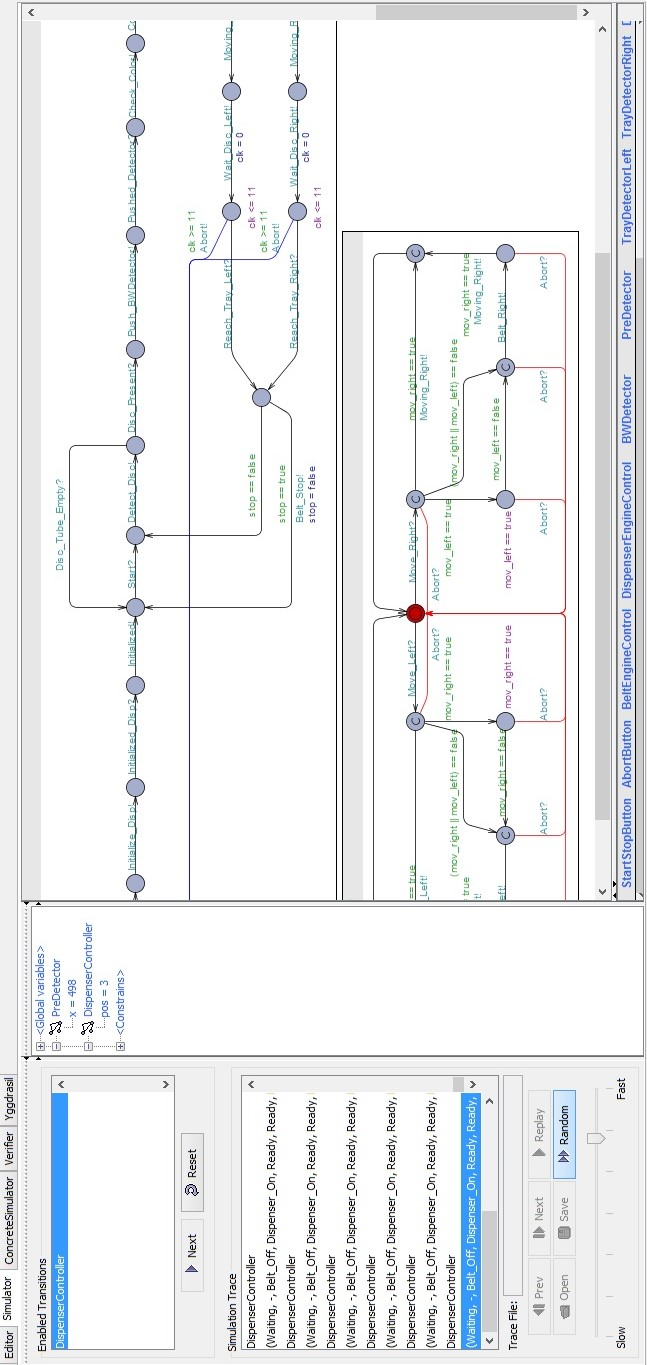
\includegraphics[height=0.65\textheight]{images/statementcoverage.jpg}
\caption{An illustration of simulation}
\label{fig:statementcoverage}
\end{figure}

\begin{figure}
\centering
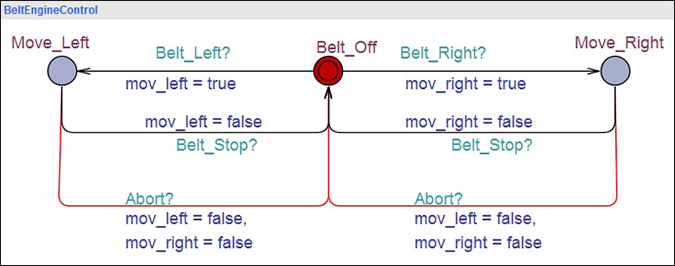
\includegraphics[width=0.9\textwidth]{images/belt1.jpg}
\caption{Resting stage of the belt}
\label{fig:belt1}
\end{figure}

\begin{figure}
\centering
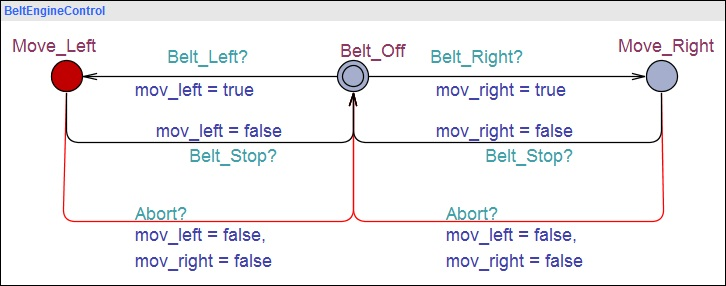
\includegraphics[width=0.9\textwidth]{images/belt2.jpg}
\caption{Belt moves to the left}
\label{fig:belt2}
\end{figure}

\begin{figure}
\centering
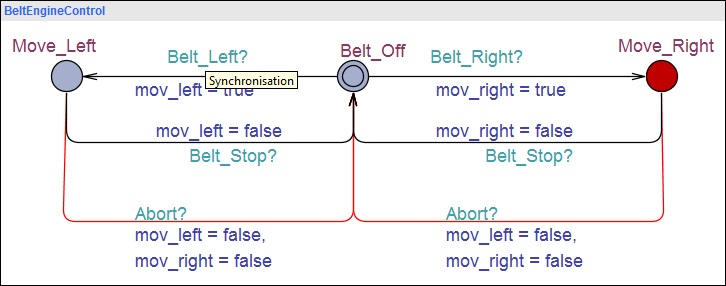
\includegraphics[width=0.9\textwidth]{images/belt3.jpg}
\caption{Belt moves to the right}
\label{fig:belt3}
\end{figure}

\begin{figure}
\centering
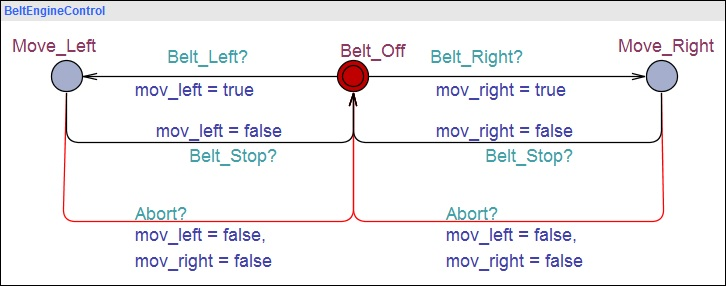
\includegraphics[width=0.9\textwidth]{images/belt4.jpg}
\caption{Belt stops}
\label{fig:belt4}
\end{figure}

\begin{figure}
\centering
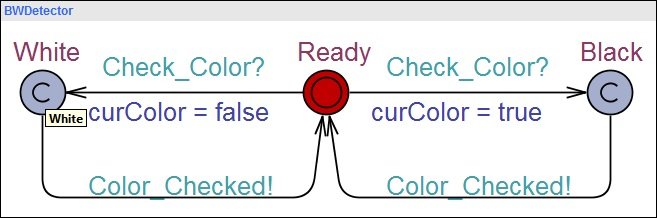
\includegraphics[width=0.9\textwidth]{images/bwd1.jpg}
\caption{Resting stage of the Black/White detector}
\label{fig:bwd1}
\end{figure}

\begin{figure}
\centering
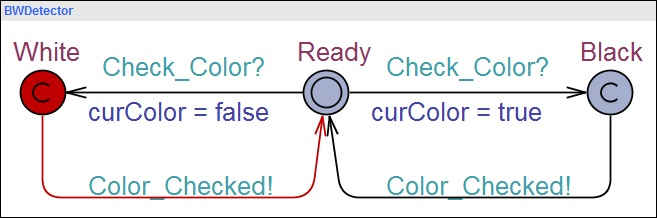
\includegraphics[width=0.9\textwidth]{images/bwd2.jpg}
\caption{A white disc has been detected}
\label{fig:bwd2}
\end{figure}

\begin{figure}
\centering
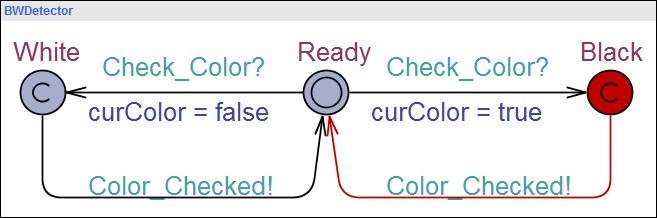
\includegraphics[width=0.9\textwidth]{images/bwd3.jpg}
\caption{A black disc has been detected}
\label{fig:bwd3}
\end{figure}

\begin{figure}
\centering
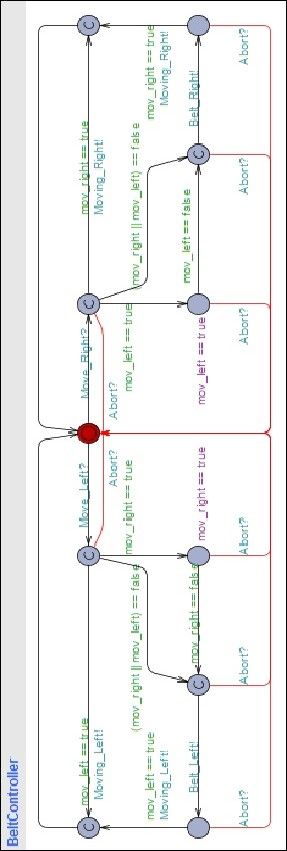
\includegraphics[height=0.75\textheight]{images/BCT1.jpg}
\caption{Resting stage of the belt controller}
\label{fig:bct1}
\end{figure}

\begin{figure}
\centering
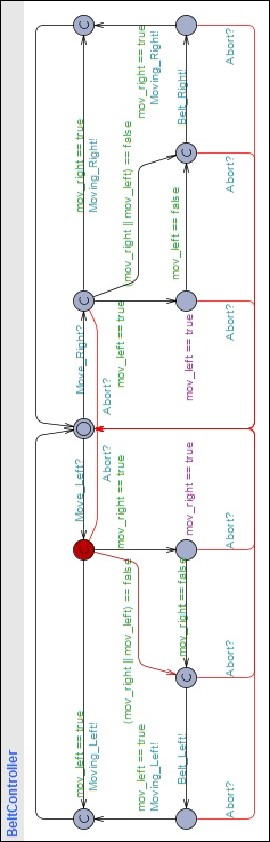
\includegraphics[height=0.75\textheight]{images/BCTL1.jpg}
\caption{An order to make belt move left}
\label{fig:bctl1}
\end{figure}

\begin{figure}
\centering
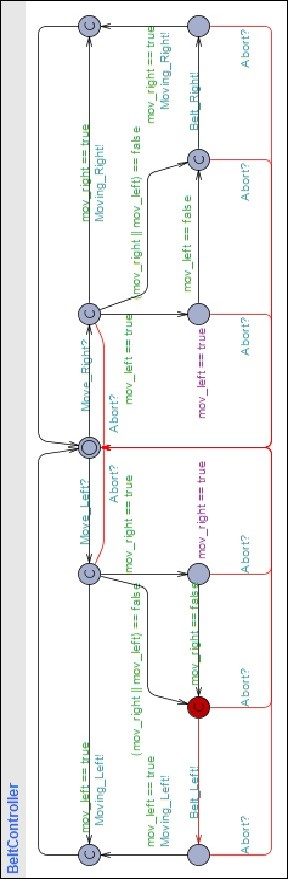
\includegraphics[height=0.75\textheight]{images/BCTL2.jpg}
\caption{Check the current direction of the belt}
\label{fig:bctl2}
\end{figure}

\begin{figure}
\centering
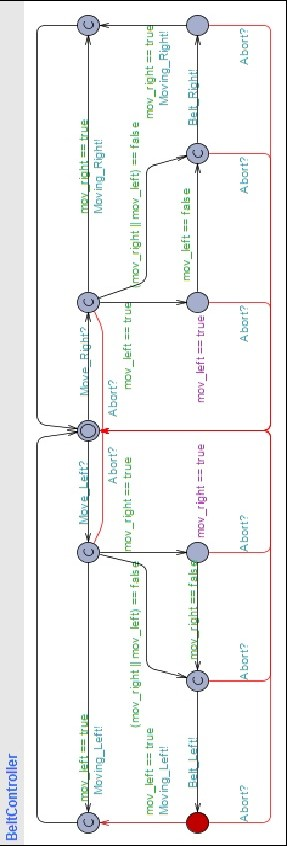
\includegraphics[height=0.75\textheight]{images/BCTL3.jpg}
\caption{Fix the boolean value}
\label{fig:bctl3}
\end{figure}

\begin{figure}
\centering
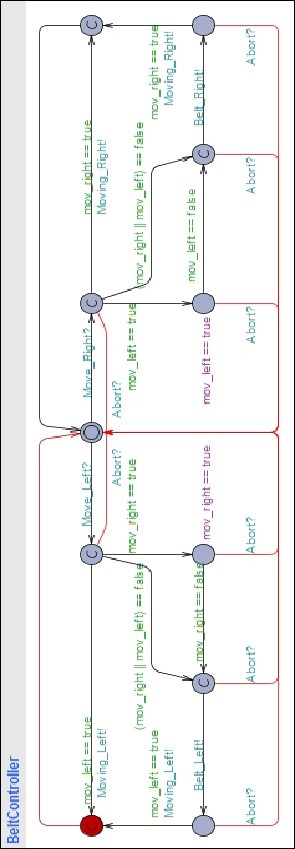
\includegraphics[height=0.75\textheight]{images/BCTL4.jpg}
\caption{Move belt to the left}
\label{fig:bctl4}
\end{figure}

\begin{figure}
\centering
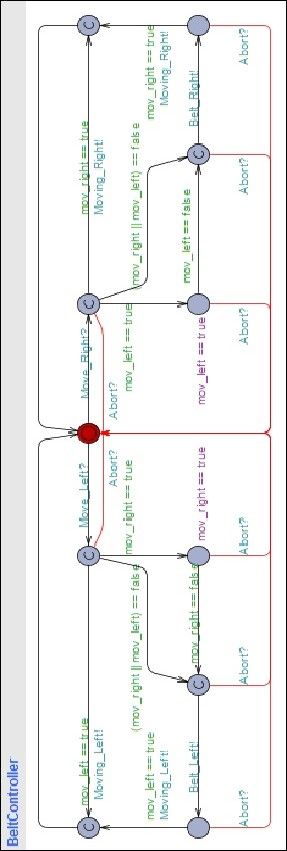
\includegraphics[height=0.75\textheight]{images/BCT1.jpg}
\caption{Movement finished}
\label{fig:bct2}
\end{figure}

\clearpage  %stop latex from crying about to much unprocessed floats, the pussy he is.

\begin{figure}
\centering
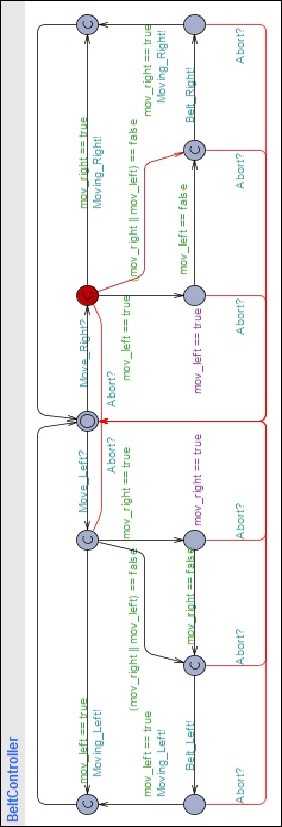
\includegraphics[height=0.75\textheight]{images/BCTR1.jpg}
\caption{An order to make belt move right}
\label{fig:bctr1}
\end{figure}

\begin{figure}
\centering
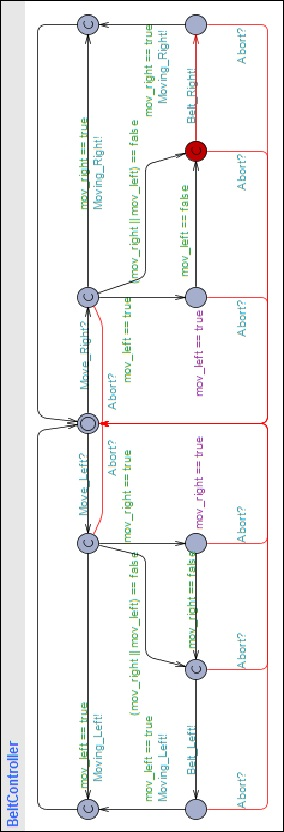
\includegraphics[height=0.75\textheight]{images/BCTR2.jpg}
\caption{Check the current direction of the belt}
\label{fig:bctr2}
\end{figure}


\begin{figure}
\centering
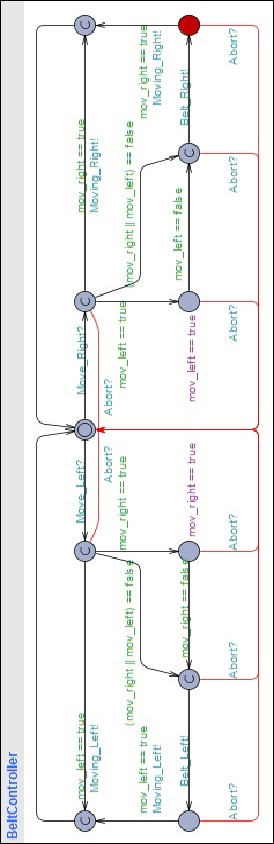
\includegraphics[height=0.75\textheight]{images/BCTR3.jpg}
\caption{Fix the boolean value}
\label{fig:bctr3}
\end{figure}

\begin{figure}
\centering
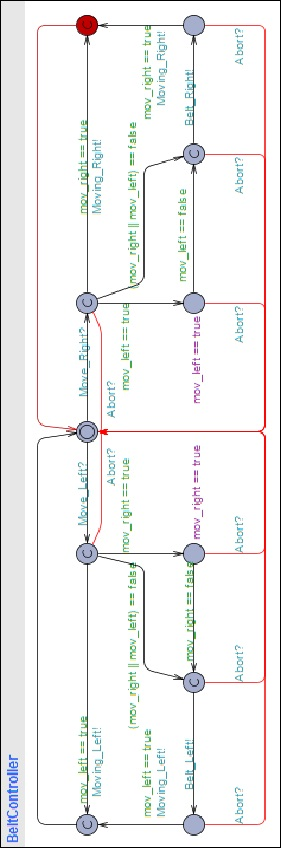
\includegraphics[height=0.75\textheight]{images/BCTR4.jpg}
\caption{Move belt to the right}
\label{fig:bctr4}
\end{figure}

\begin{figure}
\centering
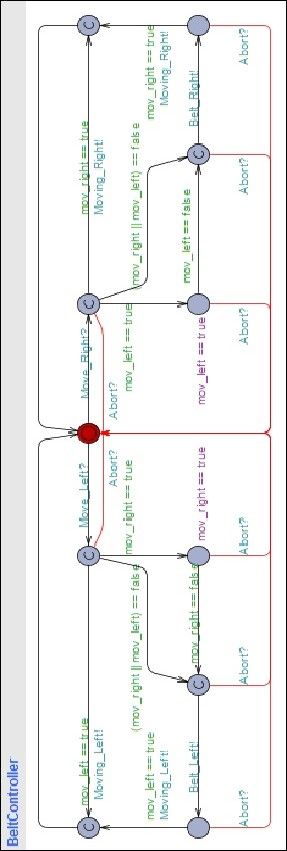
\includegraphics[height=0.75\textheight]{images/BCT1.jpg}
\caption{Movement finished}
\label{fig:bct3}
\end{figure}

\begin{figure}
\centering
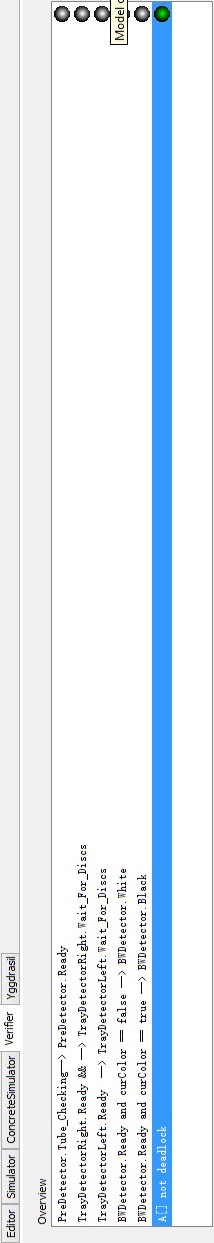
\includegraphics[height=0.75\textheight]{images/verify1.jpg}
\caption{Verifier 1: No Deadlock}
\label{fig:verify1}
\end{figure}

\begin{figure}
\centering
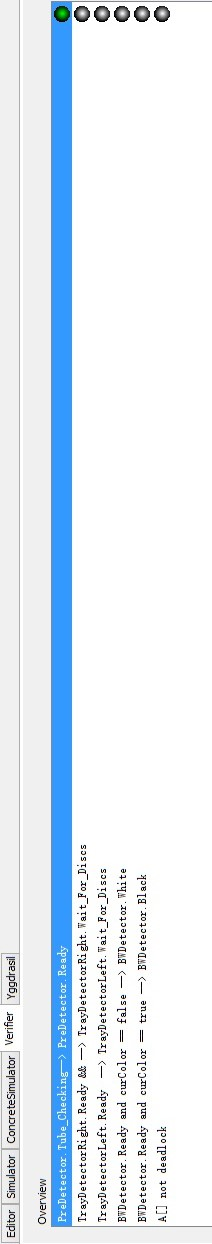
\includegraphics[height=0.75\textheight]{images/verify2.jpg}
\caption{Verifier 2: Check PreDetector}
\label{fig:verify2}
\end{figure}
\end{document} 